\documentclass{echw}

\title{Tutorial A10.2\\Complex Numbers}
\author{Eytan Chong}
\date{2024-07-05}

\begin{document}
    \problem{}
        Is the following true or false in general?

        \begin{enumerate}
            \item $\abs{w^2} = \abs{w}^2$
            \item $\abs{z + 2w} = \abs{z} + \abs{2w}$
        \end{enumerate}

    \solution
        \part
            Let $w = re^{i\t}$, where $r, \t \in \R$. Note that $\abs{e^{i\t}} = \abs{e^{2i\t}} = 1$.
            \[
                \abs{w^2} = \abs{r^2 e^{2i\t}} = r^2 \abs{e^{2i\t}} = r^2 = r^2 \abs{e^{i\t}}^2 = \abs{re^{i\t}}^2 = \abs{w}^2
            \]

            \boxt{The statement $\abs{w^2} = \abs{w}^2$ is true in general.}

        \part
            Take $z = 1$ and $w = -1$.
            \[
                \abs{z + 2w} = \abs{1 - 2} = 1 \neq 3 = \abs{1} + \abs{2 \cdot -1} = \abs{z} + \abs{2w}
            \]

            \boxt{The statement $\abs{z + 2w} = \abs{z} + \abs{2w}$ is false in general.}

    \problem{}
        Express the following complex numbers $z$ in polar form $r(\cos\t + i\sin\t)$ with exact values.

        \begin{enumerate}
            \item $z = 2-2i$
            \item $z = -1 + i\sqrt3$
            \item $z = -5i$
            \item $z = -2\sqrt3 - 2i$
        \end{enumerate}

    \solution
        \part
            \begin{center}
                \begin{tikzpicture}[trim axis left, trim axis right]
                    \begin{axis}[
                        domain = 0:10,
                        samples = 101,
                        axis y line=middle,
                        axis x line=middle,
                        xtick = {2},
                        ytick = {-2},
                        yticklabels = {$-2i$},
                        xmax=3,
                        xmin=-1,
                        ymin=-3,
                        ymax=1,
                        xlabel = {$\Re$},
                        ylabel = {$\Im$},
                        legend cell align={left},
                        legend pos=outer north east,
                        after end axis/.code={
                            \path (axis cs:0,0) 
                                node [anchor=north east] {$O$};
                            }
                        ]
            
                        \coordinate (R) at (10,0);
                        \coordinate[label=below:$Z(z)$] (Z) at (2, -2);
                        \coordinate (O) at (0, 0);
                
                        \draw (O) -- (Z);
                
                        \fill (Z) circle[radius=2.5pt];
                        \draw pic [draw, angle radius=12mm, "$\t$"] {angle = Z--O--R};
                    \end{axis}
                \end{tikzpicture}
            \end{center}

            We have $r^2 = 2^2 + (-2)^2 \implies r = 2\sqrt2$ and $\tan \t = \dfrac{-2}{2} \implies \t = -\dfrac\pi4$.

            \boxt{$2 - 2i = 2\sqrt2 \bs{\cos{-\dfrac\pi4} + i\sin{-\dfrac\pi4}}$}

        \part
            \begin{center}
                \begin{tikzpicture}[trim axis left, trim axis right]
                    \begin{axis}[
                        domain = 0:10,
                        samples = 101,
                        axis y line=middle,
                        axis x line=middle,
                        xtick = {-1},
                        ytick = {sqrt(3)},
                        yticklabels = {$\sqrt3 i$},
                        xmax=1,
                        xmin=-1.5,
                        ymin=-0.5,
                        ymax=3,
                        xlabel = {$\Re$},
                        ylabel = {$\Im$},
                        legend cell align={left},
                        legend pos=outer north east,
                        after end axis/.code={
                            \path (axis cs:0,0) 
                                node [anchor=north east] {$O$};
                            }
                        ]
            
                        \coordinate (R) at (10,0);
                        \coordinate[label=above:$Z(z)$] (Z) at (-1, 1.73);
                        \coordinate (O) at (0, 0);
                
                        \draw (O) -- (Z);
                
                        \fill (Z) circle[radius=2.5pt];
                        \draw pic [draw, angle radius=12mm, "$\t$"] {angle = R--O--Z};
                    \end{axis}
                \end{tikzpicture}
            \end{center}

            We have $r^2 = (-1)^2 + (\sqrt3)^2 \implies r = 2$ and $\tan t = \dfrac{\sqrt3}{-1} \implies \t = \dfrac23 \pi$.

            \boxt{$-1 + \sqrt3 i = 2 \bs{\cos{\dfrac23 \pi} + i\sin{\dfrac23 \pi}}$}

        \part
            \begin{center}
                \begin{tikzpicture}[trim axis left, trim axis right]
                    \begin{axis}[
                        domain = 0:10,
                        samples = 101,
                        axis y line=middle,
                        axis x line=middle,
                        xtick = \empty,
                        ytick = {-5},
                        yticklabels = {$-5i$},
                        xmax=1,
                        xmin=-1,
                        ymin=-6,
                        ymax=1,
                        xlabel = {$\Re$},
                        ylabel = {$\Im$},
                        legend cell align={left},
                        legend pos=outer north east,
                        after end axis/.code={
                            \path (axis cs:0,0) 
                                node [anchor=north east] {$O$};
                            }
                        ]
            
                        \coordinate (R) at (10,0);
                        \coordinate[label=right:$Z(z)$] (Z) at (0, -5);
                        \coordinate (O) at (0, 0);
                
                        \draw (O) -- (Z);
                
                        \fill (Z) circle[radius=2.5pt];
                        \draw pic [draw, angle radius=6mm, "$\t$"] {right angle = Z--O--R};
                    \end{axis}
                \end{tikzpicture}
            \end{center}

            We have $r = 5$ and $\t = -\dfrac\pi2$.

            \boxt{$-5i = 5\bs{\cos{-\dfrac\pi2} + i\sin{-\dfrac\pi2}}$}

        \part
            \begin{center}
                \begin{tikzpicture}[trim axis left, trim axis right]
                    \begin{axis}[
                        domain = 0:10,
                        samples = 101,
                        axis y line=middle,
                        axis x line=middle,
                        xtick = {-3.46},
                        ytick = {-2},
                        xticklabels = {$-2\sqrt3$},
                        yticklabels = {$-2i$},
                        xmax=1.5,
                        xmin=-4,
                        ymin=-3,
                        ymax=1,
                        xlabel = {$\Re$},
                        ylabel = {$\Im$},
                        legend cell align={left},
                        legend pos=outer north east,
                        after end axis/.code={
                            \path (axis cs:0,0) 
                                node [anchor=south east] {$O$};
                            }
                        ]
            
                        \coordinate (R) at (10,0);
                        \coordinate[label=above:$Z(z)$] (Z) at (-3.46, -2);
                        \coordinate (O) at (0, 0);
                
                        \draw (O) -- (Z);
                
                        \fill (Z) circle[radius=2.5pt];
                        \draw pic [draw, angle radius=12mm, "$\t$"] {angle = Z--O--R};
                    \end{axis}
                \end{tikzpicture}
            \end{center}

            We have $r^2 = (-2\sqrt3)^2 + (-2)^2 \implies r = 4$ and $\tan t = \dfrac{-2}{-2\sqrt3} \implies \t = -\dfrac56 \pi$.

            \boxt{$-2\sqrt3 - 2i = 4\bs{\cos{-\dfrac56 \pi} + i\sin{-\dfrac56 \pi}}$}

    \problem{}
        Express the following complex numbers $z$ in exponential form $re^{i\t}$.

        \begin{enumerate}
            \item $z = -1 + \dfrac2{13}i$
            \item $z = \cos 50\deg + i\sin 50\deg$
        \end{enumerate}

    \solution
        \part
            \begin{center}
                \begin{tikzpicture}[trim axis left, trim axis right]
                    \begin{axis}[
                        domain = 0:10,
                        samples = 101,
                        axis y line=middle,
                        axis x line=middle,
                        xtick = {-1},
                        ytick = {2/13},
                        yticklabels = {$\dfrac2{13}i$},
                        xmax=1,
                        xmin=-2,
                        ymin=-0.1,
                        ymax=0.2,
                        xlabel = {$\Re$},
                        ylabel = {$\Im$},
                        legend cell align={left},
                        legend pos=outer north east,
                        after end axis/.code={
                            \path (axis cs:0,0) 
                                node [anchor=north east] {$O$};
                            }
                        ]
            
                        \coordinate (R) at (10,0);
                        \coordinate[label=above:$Z(z)$] (Z) at (-1, 2/13);
                        \coordinate (O) at (0, 0);
                
                        \draw (O) -- (Z);
                
                        \fill (Z) circle[radius=2.5pt];
                        \draw pic [draw, angle radius=12mm, "$\t$"] {angle = R--O--Z};
                    \end{axis}
                \end{tikzpicture}
            \end{center}

            We have $r^2 = (-1)^2 + \bp{\dfrac2{13}}^2 \implies r = 1.02 \tosf{3}$ and $\tan t = \dfrac{2/13}{-1} \implies \t = 2.99 \tosf{3}$.

            \boxt{$-1 + \dfrac2{13}i = 1.02e^{2.99i}$}

        \part
            We have $r = 1$ and $\t = -50 \deg = -\dfrac{50}{180}\pi = -\dfrac5{18}\pi$.

            \boxt{$\cos 50 \deg + i \sin 50 \deg = e^{-i\frac5{18}\pi}$}

    \problem{}
        Express the following complex numbers $z$ in Cartesian form.

        \begin{enumerate}
            \item $z = 7e^{1 - 5i}$
            \item $z = 6\bp{\cos \dfrac\pi8 - i\sin\dfrac\pi8}$
        \end{enumerate}

    \solution
        \part
            \begin{align*}
                z &= 7e^{1-5i}\\
                &= 7e \cdot e^{-5i}\\
                &= 7e \bs{\cos{-5} + i\sin{-5}}\\
                &= 5.40 + 18.2i \tosf{3}
            \end{align*}

            \boxt{$7e^{1-5i} = 5.40 + 18.2i$}

        \part
            \begin{align*}
                z &= 6\bp{\cos \dfrac\pi8 - i\sin\dfrac\pi8}\\
                &= 5.54 - 2.30i \tosf{3}
            \end{align*}

            \boxt{$6\bp{\cos \dfrac\pi8 - i\sin\dfrac\pi8} = 5.54 - 2.30i$}

    \problem{}
        Given that $z = \sqrt3 - i$, find the exact modulus and argument of $z$. Hence, find the exact modulus and argument of $\dfrac1{z^2}$ and $z^{10}$.

    \solution
        \begin{center}
            \begin{tikzpicture}[trim axis left, trim axis right]
                \begin{axis}[
                    domain = 0:10,
                    samples = 101,
                    axis y line=middle,
                    axis x line=middle,
                    xtick = {sqrt(3)},
                    xticklabels={$\sqrt3$},
                    ytick = {-1},
                    yticklabels = {$-i$},
                    xmax=2,
                    xmin=-0.5,
                    ymin=-1.5,
                    ymax=0.5,
                    xlabel = {$\Re$},
                    ylabel = {$\Im$},
                    legend cell align={left},
                    legend pos=outer north east,
                    after end axis/.code={
                        \path (axis cs:0,0) 
                            node [anchor=north east] {$O$};
                        }
                    ]
        
                    \coordinate (R) at (10,0);
                    \coordinate[label=below:$Z(z)$] (Z) at (1.73, -1);
                    \coordinate (O) at (0, 0);
            
                    \draw (O) -- (Z);
            
                    \fill (Z) circle[radius=2.5pt];
                    \draw pic [draw, angle radius=12mm, "$\t$"] {angle = Z--O--R};
                \end{axis}
            \end{tikzpicture}
        \end{center}

        We have $r^2 = (\sqrt3)^2 + (-1)^2 \implies r = 2$ and $\tan t = \dfrac{-1}{\sqrt3} \implies \t = -\dfrac\pi6$.

        \boxt{$\abs{z} = 2$, $\arg z = -\dfrac\pi6$}

        Note that $\abs{\dfrac1{z^2}} = \abs{z}^{-2} = 2^{-2} = \dfrac14$. Also, $\arg{\dfrac1{z^2}} = -2 \arg z = -2 \cdot -\dfrac\pi6 = \dfrac\pi3$.

        \boxt{$\abs{\dfrac1{z^2}} = \dfrac14$, $\arg{\dfrac1{z^2}} = \dfrac\pi3$}

        Note that$\abs{z^{10}} = \abs{z}^10 = 2^10 = 1024$. Also, $\arg z^{10} = 10 \arg z = 10 \cdot -\dfrac\pi6 = -\dfrac53\pi \equiv \dfrac\pi3$.

        \boxt{$\abs{z^{10}} = 1024$, $\arg{z^{10}} = \dfrac\pi3$}

    \problem{}
        If $\arg{z - \dfrac12} = \dfrac\pi5$, determine $\arg{2z - 1}$.

    \solution
        \[
            \arg{2z - 1} = \arg{\dfrac12 \bs{z - \dfrac12}} = \arg{z - \dfrac12} = \dfrac\pi5
        \]

        \boxt{$\arg{2z - 1} = \dfrac\pi5$}


    \problem{}
        In an Argand diagram, points $P$ and $Q$ represent the complex numbers $z = 1 + i$ and $w = 1 + 2i$ respectively, and $O$ is the origin.

        \begin{enumerate}
            \item Mark on the Argand diagram the points $P$ and $Q$, and the points $R$ and $S$ which represent $z + w$ and $iw$ respectively.
            \item What is the geometrical shape of $OPRQ$?
            \item State the angle $SOP$.
        \end{enumerate}

    \solution
        \part
            \begin{center}
                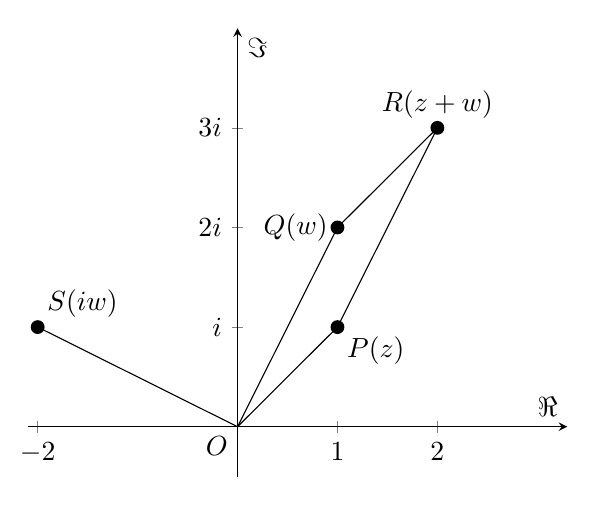
\begin{tikzpicture}[trim axis left, trim axis right]
                    \begin{axis}[
                        domain = 0:10,
                        samples = 101,
                        axis y line=middle,
                        axis x line=middle,
                        xtick = {-2, 1, 2},
                        ytick = {1, 2, 3},
                        yticklabels = {$i$, $2i$, $3i$},
                        xmax=3.3,
                        xmin=-2.1,
                        ymin=-0.5,
                        ymax=4,
                        xlabel = {$\Re$},
                        ylabel = {$\Im$},
                        legend cell align={left},
                        legend pos=outer north east,
                        after end axis/.code={
                            \path (axis cs:0,0) 
                                node [anchor=north east] {$O$};
                            }
                        ]
            
                        \coordinate (R) at (10,0);
                        \coordinate[label=below right:$P(z)$] (P) at (1, 1);
                        \coordinate[label=left:$Q(w)$] (Q) at (1, 2);
                        \coordinate[label=above:$R(z+w)$] (R) at (2, 3);
                        \coordinate[label=above right:$S(iw)$] (S) at (-2, 1);
                        \coordinate (O) at (0, 0);
                
                        \draw (O) -- (P);
                        \draw (O) -- (Q);
                        \draw (Q) -- (R);
                        \draw (P) -- (R);
                        \draw (O) -- (S);
                
                        \fill (P) circle[radius=2.5pt];
                        \fill (Q) circle[radius=2.5pt];
                        \fill (R) circle[radius=2.5pt];
                        \fill (S) circle[radius=2.5pt];
                    \end{axis}
                \end{tikzpicture}
            \end{center}

        \part
            \boxt{$OPRQ$ is a parallelogram.}

        \part
            \boxt{$\angle SOP = \dfrac\pi2$}

    \problem{}
        $B$ and $D$ are points in the Argand diagram representing the complex numbers $1 + 5i$ and $5 + 3i$ respectively. Given that $BD$ is a diagonal of the square $ABCD$, calculate the complex numbers represented by $A$ and $C$.

    \solution
        \begin{center}
            \begin{tikzpicture}[trim axis left, trim axis right]
                \begin{axis}[
                    domain = 0:10,
                    samples = 101,
                    axis y line=middle,
                    axis x line=middle,
                    xtick = {1, 5},
                    ytick = {3, 5},
                    yticklabels = {$3i$, $5i$},
                    xmax=9,
                    xmin=-1,
                    ymin=-1,
                    ymax=8,
                    xlabel = {$\Re$},
                    ylabel = {$\Im$},
                    legend cell align={left},
                    legend pos=outer north east,
                    after end axis/.code={
                        \path (axis cs:0,0) 
                            node [anchor=north east] {$O$};
                        }
                    ]
        
                    \coordinate (R) at (10,0);
                    \coordinate[label=below:$A$] (A) at (2, 2);
                    \coordinate[label=left:$B$] (B) at (1, 5);
                    \coordinate[label=above:$C$] (C) at (4, 6);
                    \coordinate[label=right:$D$] (D) at (5, 3);
                    \coordinate (O) at (0, 0);

                    \draw (A) -- (B);
                    \draw (B) -- (C);
                    \draw (C) -- (D);
                    \draw (D) -- (A);
                        
                    \fill (A) circle[radius=2.5pt];
                    \fill (B) circle[radius=2.5pt];
                    \fill (C) circle[radius=2.5pt];
                    \fill (D) circle[radius=2.5pt];
                \end{axis}
            \end{tikzpicture}
        \end{center}

        Let $A(x + iy)$. Since $AB \perp AD$, we have $b - a = i(d - a)$.
        \begin{alignat*}{2}
            && b - a &= i(d - a)\\
            \implies&& (1 + 5i) - (x + iy) &= i\bs{(5 + 3i) - (x + iy)}\\
            \implies&& (1 - x) + (5 - y)i &= (-3 + y) + (5 - x)i\\
            \implies&&(x + y) + (y - x)i &= 4
        \end{alignat*}
        Comparing real and imaginary parts, we obtain $x = y = 2$. Hence, $A(2 + 2i)$.

        Let $C(u + iv)$. Since $CB \perp CD$, we have $d - c = i(b - c)$.
        \begin{alignat*}{2}
            && d - c &= i(b - c)\\
            \implies&&(5 + 3i) - (u + iv) &= i\bs{(1 + 5i) - (u + iv)}\\
            \implies&& (5 - u) + (3 - v)i &= (-5 + v) + (1 - u)i\\
            \implies&& (u + v) + (v - u)i &= 10 + 2i
        \end{alignat*}
        Comparing real and imaginary parts, we obtain $u = 4$ and $v = 6$. Hence, $C(4 + 6i)$.

        \boxt{$A(2 + 2i)$, $C(4 + 6i)$}
    \problem{}
        \begin{enumerate}
            \item Given that $u = 2\bp{\cos\dfrac\pi6 + i\sin\dfrac\pi6}$ and $w = 4\bp{\cos\dfrac\pi3 - i\sin\dfrac\pi3}$, find the modulus and argument of $\dfrac{u\cconj}{w^3}$ in exact form.
            \item Let $z$ be the complex number $-1 + i\sqrt3$. Find the value of the real number $a$ such that $\arg{z^2 + az} = -\dfrac\pi2$.
        \end{enumerate}

    \solution
        \part
            Note that $\abs{u} = 2$, $\arg u = \dfrac\pi6$, $\abs{w} = 4$ and $\arg w = -\dfrac\pi3$.
            \[
                \abs{\dfrac{u\cconj}{w^3}} = \dfrac{\abs{u\cconj}}{\abs{w^3}} = \dfrac{\abs{u}}{\abs{w}^3} = \dfrac{2}{4^3} = \dfrac1{32}
            \]
            \[
                \arg \dfrac{u\cconj}{w^3} = \arg u\cconj - \arg w^3 = -\arg u - 3\arg w = -\dfrac\pi6 - 3 \cdot -\dfrac\pi3 = \dfrac56 \pi
            \]

            \boxt{$\abs{\dfrac{u\cconj}{w^3}} = \dfrac1{32}$, $\arg \dfrac{u\cconj}{w^3} = \dfrac56\pi$}

        \part
            Since $\arg{z^2 + az} = -\dfrac\pi2$, we have that $z^2 + az$ is purely imaginary, with a negative imaginary part. Note that $z^2 = (-1 + i\sqrt3)^2 = -2 -2\sqrt3 i$.
            \begin{alignat*}{2}
                &&\Re{z^2 + az} &= 0\\
                \implies&&\Re{(-2 - 2\sqrt3i) + a(-1 + i\sqrt3)} &= 0\\
                \implies&&-2 -a &= 0\\
                \implies&&a &= -2
            \end{alignat*}

            \boxt{$a = -2$}

    \problem{}
        The complex number $w$ has modulus $r$ and argument $\t$, where $0 < \t < \pi/2$, and $w\cconj$ denotes the conjugate of $w$. State the modulus and argument of $p$, where $p = \dfrac{w}{w\cconj}$. Given that $p^5$ is real and positive, find the possible values of $\t$.

    \solution
        \boxt{$\abs{p} = 1$, $\arg p = 2\t$}

        Since $p^5 = 0$, we have $\arg p^5 = 2\pi n$, where $n \in \mathbb{Z}$. Thus, $\arg p = \dfrac{2\pi n}5 = 2\t \implies \t = \dfrac{\pi n}{5}$. Since $0 < \t < \dfrac\pi2$, the possible values of $\t$ are $\dfrac15 \pi$ and $\dfrac25 \pi$.

        \boxt{$\t = \dfrac15 \pi, \dfrac25\pi$}

    \problem{}
        The complex number $w$ has modulus $\sqrt2$ and argument $-\dfrac34\pi$, and the complex number $z$ has modulus 2 and argument $-\dfrac\pi3$. Find the modulus and argument of $wz$, giving each answer exactly.

        By first expressing $w$ and $z$ in the form $x + iy$, find the exact real and imaginary parts of $wz$.

        Hence, show that $\sin \dfrac\pi{12} = \dfrac{\sqrt3 - 1}{2\sqrt2}$.

    \solution
        \[
            \abs{wz} = \abs{w} \abs{z} = 2\sqrt2
        \]
        \[
            \arg{wz} = \arg w + \arg z = - \dfrac34 \pi - \dfrac13 \pi = -\dfrac{13}{12}\pi \equiv \dfrac{11}{12} \pi
        \]
        \boxt{$\abs{wz} = 2\sqrt2$, $\arg{wz} = \dfrac{11}{12}\pi$}

        \[
            w = \sqrt2 \bs{\cos{-\dfrac34 \pi} + i\sin{-\dfrac34 \pi}} = \sqrt2 \bp{-\dfrac1{\sqrt2} - \dfrac1{\sqrt2} i} = -1-i
        \]
        \[
            z = 2\bs{\cos{-\dfrac\pi3} + i\sin{-\dfrac\pi3}} = 2\bp{\dfrac12 - \dfrac{\sqrt3}{2} i} = 1 - \sqrt3 i
        \]
        \[
            \implies wz = (-1 - i)(1 - \sqrt3 i) = (-1 + \sqrt3 -i - \sqrt3) = (-1 - \sqrt3) + (\sqrt3 - 1)i
        \]
        \boxt{$\Re{wz} = -1 - \sqrt3$, $\Im{wz} = \sqrt3 - 1$}

        From the first part, we have that $wz = 2\sqrt2 \bs{\cos{\dfrac{11}{12} \pi} + i\sin{\dfrac{11}{12} \pi}}$. Thus, $\Im{wz} = 2\sqrt{2} \sin{\dfrac{11}{12} \pi} = 2\sqrt2 \sin \dfrac\pi{12}$. Equating the result for $\Im{wz}$ found in the second part, we have $2\sqrt2 \sin \dfrac\pi{12} = \sqrt3 - 1 \implies \sin \dfrac{\pi}{12} = \dfrac{\sqrt3 - 1}{2\sqrt2}$.
    \problem{}
        Given that $\dfrac{5 + z}{5 - z} = e^{i\t}$, show that $z$ can be written as $5i\tan\dfrac\t2$.

    \solution
        Note that $\dfrac{5 + z}{5 - z} = e^{i\t} \implies 5 + z = e^{i\t} (5-z) \implies z + e^{i\t}z = 5e^{i\t} - 5 \implies z = 5 \cdot \dfrac{e^{i\t} - 1}{e^{i\t} + 1}$.
        \begin{align*}
            z &= 5 \cdot \dfrac{e^{i\t} - 1}{e^{i\t} + 1}\\
            &= 5 \cdot \dfrac{\cos\t + i\sin\t - 1}{\cos\t + i\sin\t + 1}\\
            &= 5 \cdot \dfrac{\bs{\cos[2]{\t/2} - \sin[2]{\t/2}} + i\bs{2\sin{\t/2}\cos{\t/2}} - \bs{\cos[2]{\t/2} + \sin[2]{\t/2}}}{\bs{\cos[2]{\t/2} - \sin[2]{\t/2}} + i\bs{2\sin{\t/2}\cos{\t/2}} + \bs{\cos[2]{\t/2} + \sin[2]{\t/2}}}\\
            &= 5 \cdot \dfrac{-2\sin[2]{\t/2} + 2i\sin{\t/2}\cos{\t/2}}{2\cos[2]{\t/2} + 2i\sin{\t/2}\cos{\t/2}}\\
            &= 5 \cdot \dfrac{-\sin[2]{\t/2} + i\sin{\t/2}\cos{\t/2}}{\cos[2]{\t/2} + i\sin{\t/2}\cos{\t/2}}\\
            &= 5 \cdot \dfrac{-\tan{\t/2} + i}{\cot{\t/2} + i}\\
            &= 5 \cdot \dfrac{i^2\tan{\t/2} + i\tan{\t/2}\cot{\t/2}}{\cot{\t/2} + i}\\
            &= 5 \cdot \dfrac{i\tan{\t/2} \bs{i + \cot{\t/2}}}{\cot{\t/2} + i}\\
            &= 5i\tan \dfrac\t2
        \end{align*}

    \problem{}
        The polynomial $P(z)$ has real coefficients. The equation $P(z) = 0$ has a root $re^{i\t}$, where $r > 0$ and $0 < \t < \pi$.

        \begin{enumerate}
            \item Write down a second root in terms of $r$ and $\t$, and hence show that a quadratic factor of $P(z)$ is $z^2 - 2rz\cos\t + r^2$.
            \item Given that 3 roots of the equation $z^6 = -64$ are $2e^{i \frac\pi6}$, $2e^{i\frac\pi2}$ and $2e^{-i\frac{5\pi}6}$, express $z^6 + 64$ as a product of three quadratic factors with real coefficients, giving each factor in non-trigonometric form.
            \item Represent all roots of $z^6 = -64$ on an Argand diagram and interpret the geometrical shape formed by joining the roots.
        \end{enumerate}

    \solution
        \part
            Since $P(z)$ has real coefficients, $(re^{i\t})\cconj = re^{-i\t}$ is also a root of $P(z)$.

            \boxt{A second root is $re^{-i\t}$.}
            \begin{align*}
                P(z) &= Q(z)(z - re^{i\t})(z - re^{-i\t})\\
                &= Q(z)(z^2 -rz(e^{i\t} + e^{-i\t}) + r^2e^{i\t}e^{-i\t})\\
                &= Q(z)(z^2 - rz \cdot 2 \Re{e^{i\t}} + r^2)\\
                &= Q(z)(z^2 - 2rz\cos\t + r^2)
            \end{align*}

        \part
            Let $r_1 = r_2 = r_3 = 2$ and $\t_1 = \dfrac\pi6$, $\t_2 = \dfrac\pi2$ and $\t_3 = -\dfrac56 \pi$.
            \begin{align*}
                z^6 + 64 &= \bp{z^2 - 2r_1z\cos\t_1 + r_1^2}\bp{z^2 - 2r_2z\cos\t_2 + r_2^2}\bp{z^2 - 2r_3z\cos\t_3 + r_3^2}\\
                &= \bp{z^2 - 4z\cos{\dfrac\pi6} + 4}\bp{z^2 - 4z\cos{\dfrac\pi2} + 4} \bp{z^2 - 4z\cos{-\dfrac56 \pi} + 4}\\
                &= \bp{z^2 - 2\sqrt3 z + 4}\bp{z^2 + 4} \bp{z^2 + 2\sqrt3 z + 4}
            \end{align*}

            \boxt{$z^6 + 64 = \bp{z^2 - 2\sqrt3 z + 4}\bp{z^2 + 4} \bp{z^2 + 2\sqrt3 z + 4}$}

        \part
            \begin{center}
                \begin{tikzpicture}[trim axis left, trim axis right]
                    \begin{axis}[
                        domain = 0:10,
                        samples = 101,
                        axis y line=middle,
                        axis x line=middle,
                        xtick = \empty,
                        ytick = \empty,
                        xmax=3.3,
                        xmin=-3.3,
                        ymin=-3.3,
                        ymax=3.3,
                        xlabel = {$\Re$},
                        ylabel = {$\Im$},
                        legend cell align={left},
                        legend pos=outer north east,
                        after end axis/.code={
                            \path (axis cs:0,0) 
                                node [anchor=north east] {$O$};
                            }
                        ]
            
                        \coordinate (R) at (10,0);
                        \coordinate[label=right:$Z_1$] (Z1) at (1.73, 1);
                        \coordinate[label=above right:$Z_2$] (Z2) at (0, 2);
                        \coordinate[label=left:$Z_3$] (Z3) at (-1.73, 1);
                        \coordinate[label=left:$Z_4$] (Z4) at (-1.73, -1);
                        \coordinate[label=below right:$Z_5$] (Z5) at (0, -2);
                        \coordinate[label=right:$Z_6$] (Z6) at (1.73, -1);
                        \coordinate (O) at (0, 0);

                        \draw (Z1) -- (Z2);
                        \draw (Z2) -- (Z3);
                        \draw (Z3) -- (Z4);
                        \draw (Z4) -- (Z5);
                        \draw (Z5) -- (Z6);
                        \draw (Z6) -- (Z1);
                                
                        \fill (Z1) circle[radius=2.5pt];
                        \fill (Z2) circle[radius=2.5pt];
                        \fill (Z3) circle[radius=2.5pt];
                        \fill (Z4) circle[radius=2.5pt];
                        \fill (Z5) circle[radius=2.5pt];
                        \fill (Z6) circle[radius=2.5pt];
                    \end{axis}
                \end{tikzpicture}
            \end{center}

            \boxt{The geometrical shape formed is a regular hexagon.}
\end{document}